\section{Geometric adapter implementation and earlier evaluation}
\label{app:quality-complete}
\cohortline{LOCAL ADAPTATION / 2,608 fitting queries / 434 corrected evaluation queries / historical exposure retained}

The base fusion model supplies several estimates of the same signed quantity: its final fused TTC, the RGB context estimate, and the event context estimate. Their errors need not agree, and their reliability changes with temporal support and apparent motion. PHASE-TTC-Adapt leaves all nine upstream components frozen and learns a small router over those three outputs and a causal box-expansion estimate. The experiment adapts the fusion rule over fixed representations; Section~\ref{sec:canonical-cadence} evaluates temporal normalization as a separate intervention. \evidence{N01}

The adapter uses the frozen base model, denoted F0 in the source archive. Earlier fine-tuned heads and quality-gate candidates are separate models; Appendix~\ref{app:adaptation-lineage} documents their populations, unsuccessful controls, and interval coverage. In particular, the delivered router does not use the fine-tuned weights affected by the earlier target-source assignment.

\subsection{Causal box geometry and its quality descriptors}
For each query, the geometric branch admits supplied boxes with timestamps in the preceding 650\,ms, rejects nonfinite or nonpositive extents, and requires strictly increasing observation times. It fits three apparent sizes: width, height, and square root of area. Let $s_i$ denote one such size, $s_n$ its latest value, and $u_i$ time relative to the query in seconds. The branch constructs $\rho_i=s_n/s_i$ and estimates a line using median pair slopes,
\begin{align}
 b &= \operatorname{median}_{i<j}\frac{\rho_j-\rho_i}{u_j-u_i},
 &a &= \operatorname{median}_i(\rho_i-bu_i),\\
 q_s&=-b/a \quad (a>0).
\end{align}
The median of the three $q_s$ values supplies the geometric inverse TTC. This is an apparent-scale model with a query-time intercept; it does not recover metric depth or compensate for arbitrary rotation, occlusion, or annotation jitter. At least two boxes spanning 10\,ms are needed for a fit. Near-zero expansion, nonfinite descriptors, or an endpoint older than 150\,ms makes the geometric estimate unavailable. A two-point zero residual is not interpreted as zero uncertainty. \evidence{N01}

Twenty descriptors expose the conditions of that fit: the three axis/area rates, their median and short-history counterpart, rate disagreement, residual and residual-to-motion ratio, temporal span, normalized box count, admitted-box fraction, endpoint age, quantization support, short/long disagreement, aspect ratio and its change, center motion, and slope scatter. Absolute coordinates and absolute clock time are absent. We use supplied object regions to evaluate the fusion rule under known localization. Autonomous deployment will require testing a causal detector together with the estimator, including the effects of its box errors and delay.

The intersensor projection uses calibrated rotation without depth-dependent translation, and Slider extrinsics remain provisional. The annotated-region contract and these projection limits also apply to the adaptation comparison; they should accompany any interpretation of its geometric input. \evidence{A03,A07}

\subsection{Router architecture and exact output policy}
Each quality router receives 33 values. Thirteen describe the three neural magnitudes, their availability, pairwise sign agreements, geometric availability, and neural/geometric sign agreement. The remaining twenty are the geometric quality descriptors, with the first five rate coordinates replaced by their magnitudes. This design lets the weights respond to agreement and support without supplying a sequence identifier or a target-derived error. After fitted normalization and componentwise clipping to $[-8,8]$, the gate computes $g(\mathbf x)=W_2\tanh(W_1\mathbf x+\mathbf b_1)+\mathbf b_2$, with hidden width 18 and four output logits. Its two affine maps contain 688 trainable parameters. The final affine weights start at zero with bias $(2,0,0,0)$, favoring F0 when other experts are available without forcing an exact initial F0 output. \evidence{N01}

Let $m_j$ indicate an available expert and let $g_j(\mathbf x)$ be its gate logit. The router forms normalized masked weights
\begin{equation}
 w_j=\frac{m_j\exp g_j(\mathbf x)}{\sum_k m_k\exp g_k(\mathbf x)},
 \qquad \widehat q=\sum_{j:m_j=1}\frac{w_j}{\widetilde T_j},
 \label{eq:adapt-inverse-fusion}
\end{equation}
where $\widetilde T_j$ preserves the expert sign and limits its magnitude to $[0.1,60]$\,s. The implementation excludes zero-valued experts from inverse-coordinate fusion. It applies a rate-magnitude floor of $1/60$\,s$^{-1}$ before inversion, yielding a finite signed output with magnitude at most 60\,s. Exact cancellation, $\widehat q=0$, returns the original fused prediction F0 rather than choosing an approach direction.

The delivered ensemble contains routers trained with three random seeds, for $3\times688=2,064$ learned router parameters. Each router performs Equation~\ref{eq:adapt-inverse-fusion} and emits seconds; the ensemble then averages those three TTC predictions in seconds. It does not average their inverse rates. The ensemble returns F0 exactly when no valid box history is supplied, when endpoint age is nonfinite, or when the latest box is older than 150\,ms. A valid geometric estimate is a separate requirement: a fresh but too-short box history can leave geometry unavailable while allowing the router to combine available neural estimates. These distinctions preserve the implemented fallback semantics. \evidence{N01}

\subsection{Fitting and local evaluation}
The router fit uses 2,608 queries: 2,531 from twenty-four road recordings and 77 from Slider-500. Each of three seeds runs 300 AdamW updates with learning rate and weight decay both 0.01. The evaluation recordings are excluded from these optimizer updates, but they informed earlier development; the comparison therefore measures local adaptation under the protocol in Section~\ref{sec:protocol}.

\subsection{Corrected evaluation of the delivered adapter}
\EvidenceAdaptTable
The evaluation contains 434 corrected target correspondences. We report both signed runtime predictions and the organizer-described offline interpolation of negative outputs. The latter may use later valid predictions and is never part of the causal forward path. Appendix~\ref{app:target-association} and the source records document target correction; the scoring policy is fixed in Section~\ref{sec:protocol}. \evidence{N01}

Both scoring contracts favor the adapter. With the original signed outputs retained, F0/adapted MAE is 0.8244/0.3470\,s and RAE is 49.73/17.79\%. After organizer-style interpolation, the corresponding pairs are 0.8250/0.3359\,s and 49.89/17.25\%. The MAE reductions are 57.91\% and 59.28\%, respectively.  \evidence{N01}

Over all 434 queries, MAE decreases from 0.8250 to 0.3359\,s and mean relative error from 49.89\% to 17.25\%. The respective relative reductions are 59.28\% and 65.43\%. Both errors decrease in each of the ten sequences under this evaluator. On the 365 road queries, MAE falls from 0.3054 to 0.1852\,s, showing improvement across the road domain as well as the pooled population. These query-weighted reductions use a different aggregation from the recording-macro cadence summaries in Appendix~\ref{sec:canonical-cadence}.

\begin{figure}[htbp]
\centering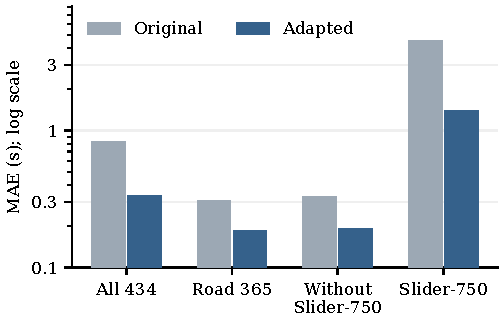
\includegraphics[width=.72\linewidth]{updates/figures/adaptation.pdf}
\caption{\textbf{Local effect of quality adaptation.} The corrected evaluator compares the original and adapted outputs on the same queries. A logarithmic vertical axis separates the road and Slider error scales. This figure reports exposed development evidence, with organizer-style negative-output interpolation applied to both variants. \evidence{N01}}
\label{fig:quality-adaptation}
\end{figure}

\paragraph{Comparison with organizer scores.}
\label{par:local-score-correspondence}
Our reconstruction matches the organizer-provided original relative error for nine of ten sequences after rounding. For Slider-750, we obtain 283.9\% rather than the organizer's 132\%; the adapted model scores 76.1\% under our local evaluator. The available records leave the source of this discrepancy unresolved. Reconciliation requires the organizer-aligned targets and exact evaluator version, so we report the adaptation gains under the local scoring contract. Appendix~\ref{app:competition-details} records the target correspondence and evaluation boundary.


\subsection{Matched attribution follow-up}
Section~\ref{sec:quality-adaptation} adds geometry-only, fallback, fixed-mixture, and router comparisons on identical query support. The earlier protocol above is retained to distinguish raw signed inference from organizer-style offline interpolation.
\FloatBarrier
